\documentclass{beamer}

\usepackage[utf8x]{inputenc}
\usepackage[english]{babel}
\usepackage[export]{adjustbox}

\mode<presentation> {
	\usetheme{Berlin}
}

\usebackgroundtemplate {
	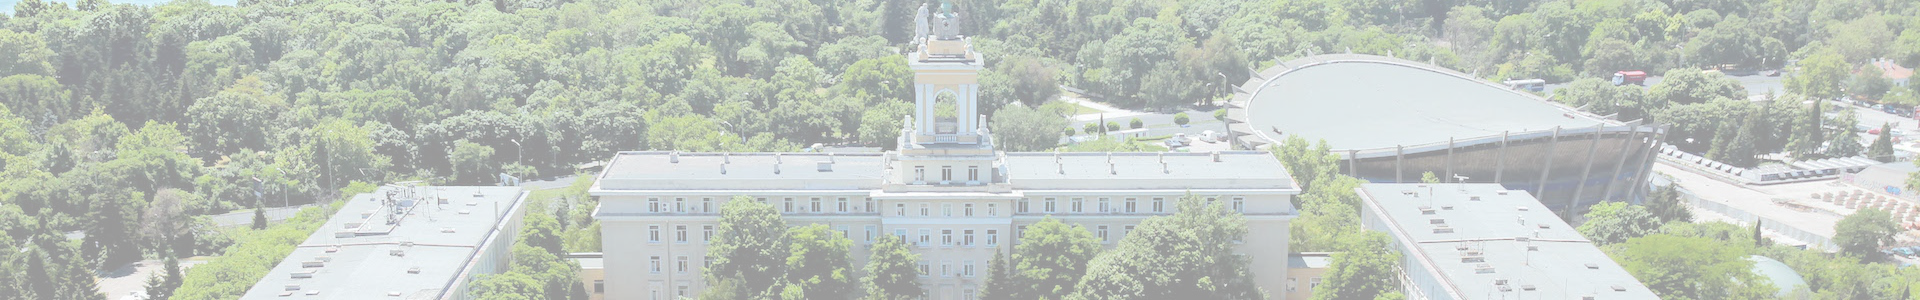
\includegraphics[width=370px, height=270px, trim=0 0 0 0px]{Snimka_MU_Varna_1.png}
}

\title[ \fontsize{5}{7}\selectfont Second International Scientific Conference Digital Transformation, Cyber Security and Resilience, September 30 - October 02, 2020, Varna, Bulgaria]{Cybersecurity in Donated Distributed Computing for Evolutionary Algorithms}

\author{Petar Tomov, Iliyan Zankinski,\\ Todor Balabanov\textsuperscript{0000-0003-3139-069X}}
%
% Bulgarian Academy of Sciences
% Institute of Information and Communication Technologies
% acad. Georgi Bonchev Str., block 2, office 514, 1113 Sofia, Bulgaria
% http://www.iict.bas.bg/
% iict@bas.bg
%

\date{30.IX-02.X.2020}

\institute[IICT-BAS, DIGILIENCE'20] {
	Institute of Information and Communication Technologies \\ 
	Bulgarian Academy of Sciences \\
	\medskip
	\textit{todorb@iinf.bas.bg}
}

\addtobeamertemplate{navigation symbols}{}{
    \usebeamerfont{footline}
    \usebeamercolor[fg]{footline}
    \hspace{1em}
    \insertframenumber/\inserttotalframenumber
}

\begin{document}

\begin{frame}
\titlepage
\end{frame}

\begin{frame}
\frametitle{Agenda}
\tableofcontents
\end{frame}

\section{Introduction}

\begin{frame}
\center \huge{Introduction}
\end{frame}

\subsection{Donated Distributed Computing}

\begin{frame}
\frametitle{Parallel Programming}
\begin{itemize}
	\item Different computation steps are not strongly connected to each other
	\item Such steps can be calculated separately
	\item Computation time is usually reduced by involving more calculating units
\end{itemize}
\end{frame}

\begin{frame}
\frametitle{Calculation Resources Ownership}
\begin{itemize}
	\item Privately owned infrastructure
	\item Usage of somebody else infrastructure
\end{itemize}
\end{frame}

\begin{frame}
\frametitle{Volunteer Computing}
\begin{itemize}
	\item Type of distributed computing
	\item People donate their computers' unused resources
	\item There is no control of any kind over the donated calculating power
\end{itemize}
\end{frame}

\begin{frame}
\frametitle{Usage Specifics}
\begin{itemize}
	\item The biggest advantage of the donated distributed computing is that it comes at a very low price
	\item The biggest disadvantage of the donated distributed computing is that it comes with a wide list of security and reliability issues
\end{itemize}
\end{frame}

\section{Evolutionary Algorithms}

\begin{frame}
\center \huge{Evolutionary Algorithms}
\end{frame}

\subsection{Metaheuristic Optimization}

\begin{frame}
\frametitle{Population Based}
\begin{itemize}
	\item Organized with some kind of population
	\item Some kind of evolution is applied
	\item Applied in global optimization problems
\end{itemize}
\end{frame}

\begin{frame}
\frametitle{Population Specifics}
\begin{itemize}
	\item Individuals are vectors into solution space
	\item Each individual is treated as a potential candidate for an optimal or sub-optimal solution
	\item Individuals are evaluated according predefined fitness function
	\item Better-fitted individuals should have better chances to mate
\end{itemize}
\end{frame}

\subsection{Optimization Problem}

\begin{frame}
\frametitle{Financial Time Series Forecasting}
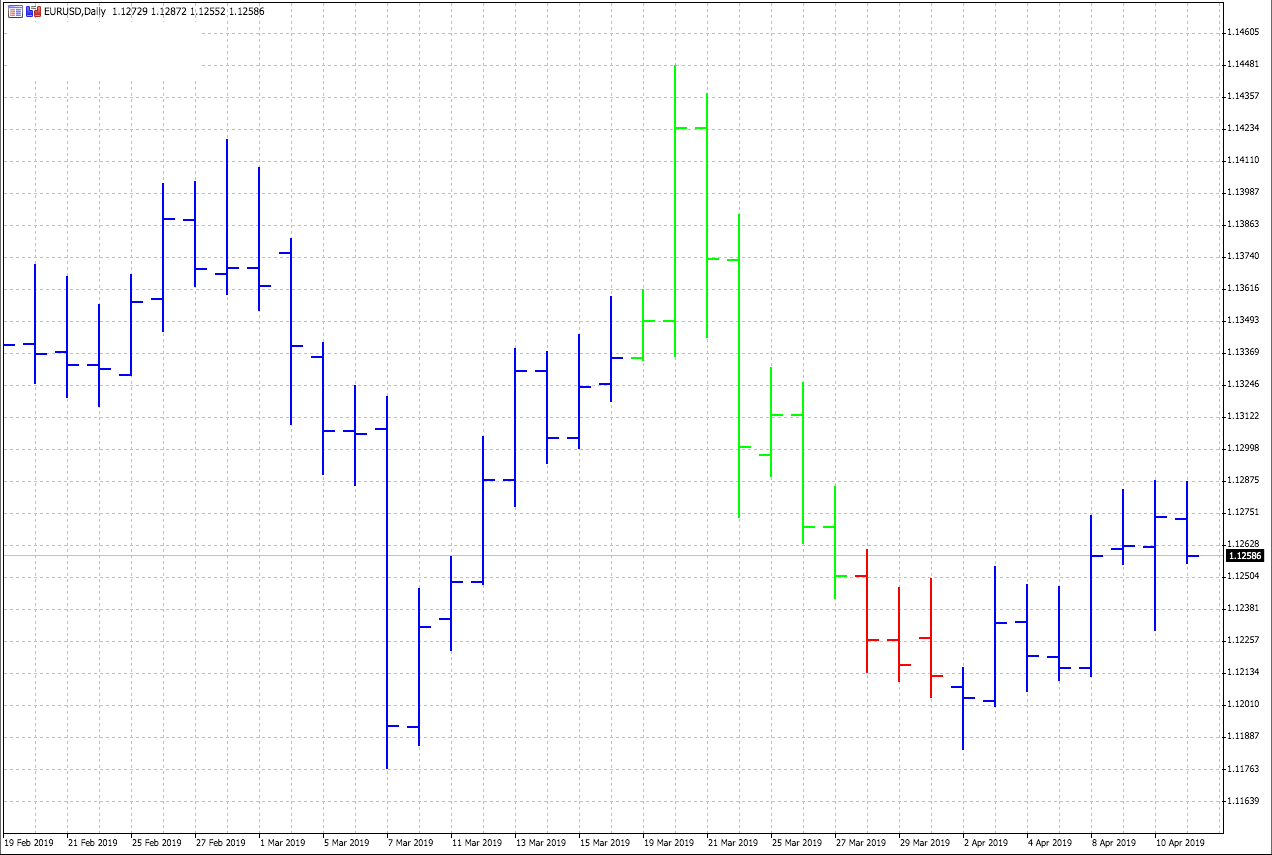
\includegraphics[scale=0.2]{fig01}
\end{frame}

\begin{frame}
\frametitle{Forecasting with Three-Layer Perceptron}
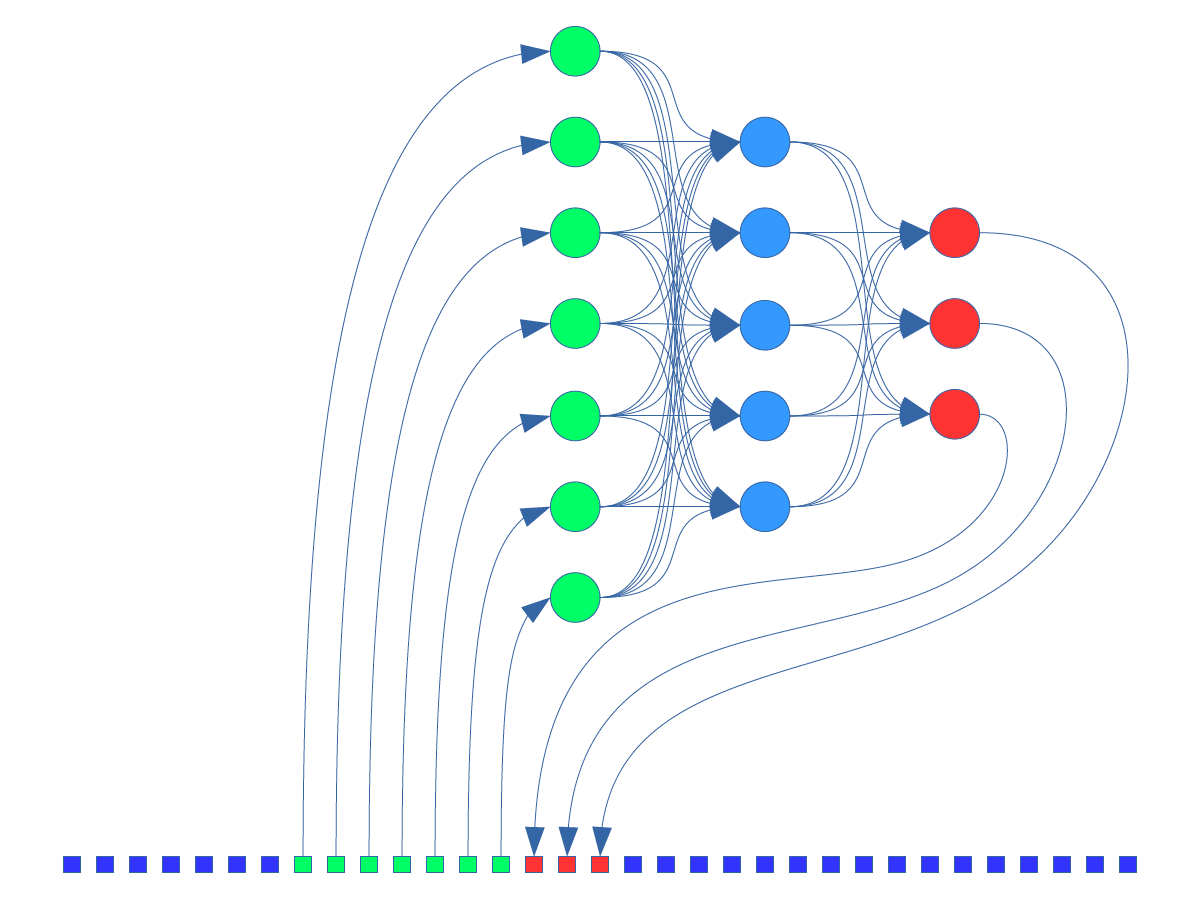
\includegraphics[scale=0.2]{fig02}
\end{frame}

\begin{frame}
\frametitle{Series as Training Set}
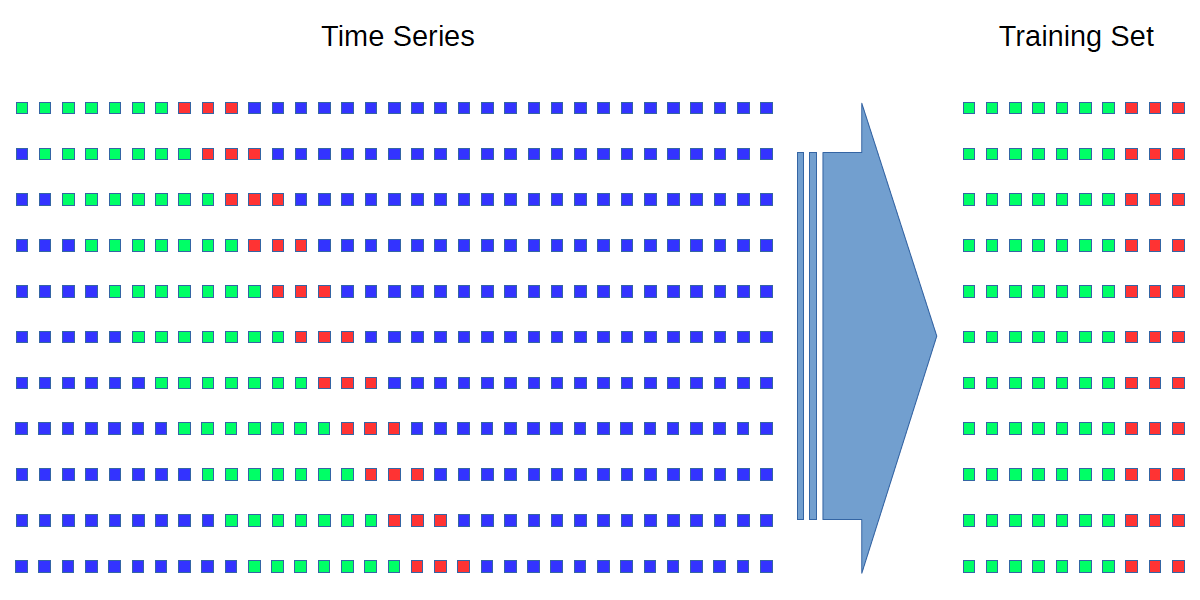
\includegraphics[scale=0.25]{fig03}
\end{frame}

\begin{frame}
\frametitle{Forecasting as Mobile Distributed Computing}
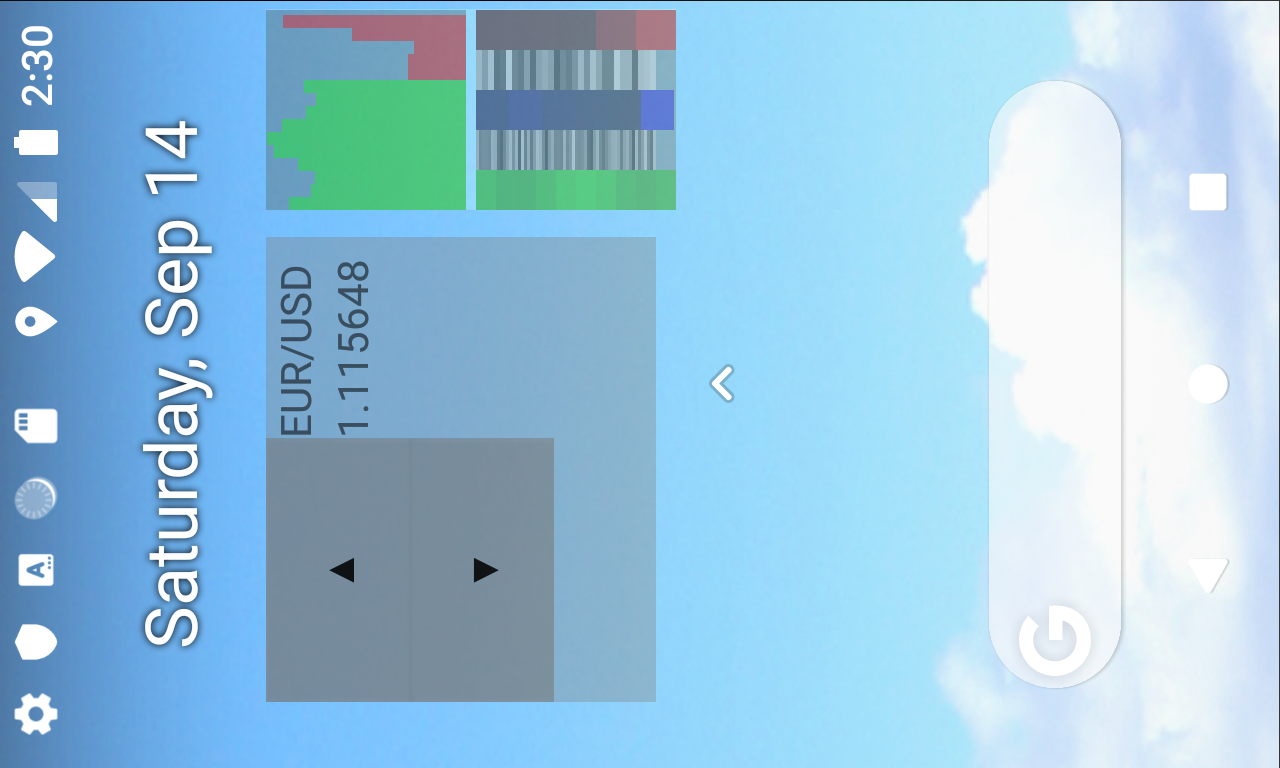
\includegraphics[scale=0.2]{fig04}
\end{frame}

\subsection{Distributed Computing Specific Security Problems}

\begin{frame}
\frametitle{General Issues}
\begin{itemize}
	\item Donated distributed computing has all security problem as the other software
	\item It has two extra security problems
	\begin{itemize}
		\item Volunteer can manipulate the calculation results
		\item The accuracy of the results are not guaranteed because of the heterogeneous hardware and software on the client-side
	\end{itemize}
\end{itemize}
\end{frame}

\begin{frame}
\frametitle{How Distributed Evolutionary Algorithms are Affected}
\begin{itemize}
	\item Fake individuals are received in the global population on the server-side
	\item Individuals with unsatisfying accuracy are received on the server-side
\end{itemize}
\end{frame}

\begin{frame}
\frametitle{The Positive Effect}
\begin{itemize}
	\item Both problems do not harm the global population so much
	\item Low-quality individuals are removed in local populations relatively fast
	\item It has even a positive effect by making genotype diversity even higher during the process of new local population forming
\end{itemize}
\end{frame}

\section{Conclusions}

\begin{frame}
\center \huge{Conclusions}
\end{frame}

\subsection{Advantages \& Disadvantages}

\begin{frame}
\frametitle{Advantages}
\begin{itemize}
	\item Cost-efficiency
	\item Almost infinite scaling capabilities
	\item Donated distributed computing is one of the most promising areas of scientific researches
	\item For population-based evolutionary algorithms some of the security issues can be even positive as a side effect than negative
\end{itemize}
\end{frame}

\begin{frame}
\frametitle{Disadvantages}
\begin{itemize}
	\item Calculations should be possible to be divided and to be done simultaneously on separate machines
\end{itemize}
\end{frame}

\begin{frame}
\frametitle{Future Research}
\begin{itemize}
	\item Investigation of cybersecurity issues if human voting is involved in fitness value estimation
\end{itemize}
\end{frame}

\subsection{Discussion}

\begin{frame}
\frametitle{Questions and Answers}
\center \huge{Thank you for your attention!}
\end{frame}

\begin{frame}
\frametitle{Acknowledgments}
This research is funded by Velbazhd Software LLC and it is partially supported by the Bulgarian Ministry of Education and Science (contract D01–205/23.11.2018) under the National Scientific Program ``Information and Communication Technologies for a Single Digital Market in Science, Education and Security (ICTinSES)'', approved by DCM \# 577/17.08.2018.
\end{frame}

\end{document}
